\section{Motivación}
\begin{frame}{Motivación}
    
   \begin{itemize}[<+->]
       \item Los modelos de Deep Learning (DL) son \textbf{determinísticos}: estimaciones puntuales de parámetros y predicciones.
       \item Los modelos actuales de DL tienden a estar \textbf{sobreparametrizados}. Ej: GPT3 ($\sim$175 bill.) Y distintos parámetros pueden ajustarse bien en entrenamiento, pero arrojan resultados distintos en prueba. 
       \item No es posible saber si el modelo está prediciendo con certeza o solo adivinando.
       \item Relevante en áreas como medicina y vehículos autónomos.
       
       
   \end{itemize}
\end{frame}

\begin{frame}{Motivación}

    \uncover<1->{
        Ejemplo: softmax.
        \begin{center}
        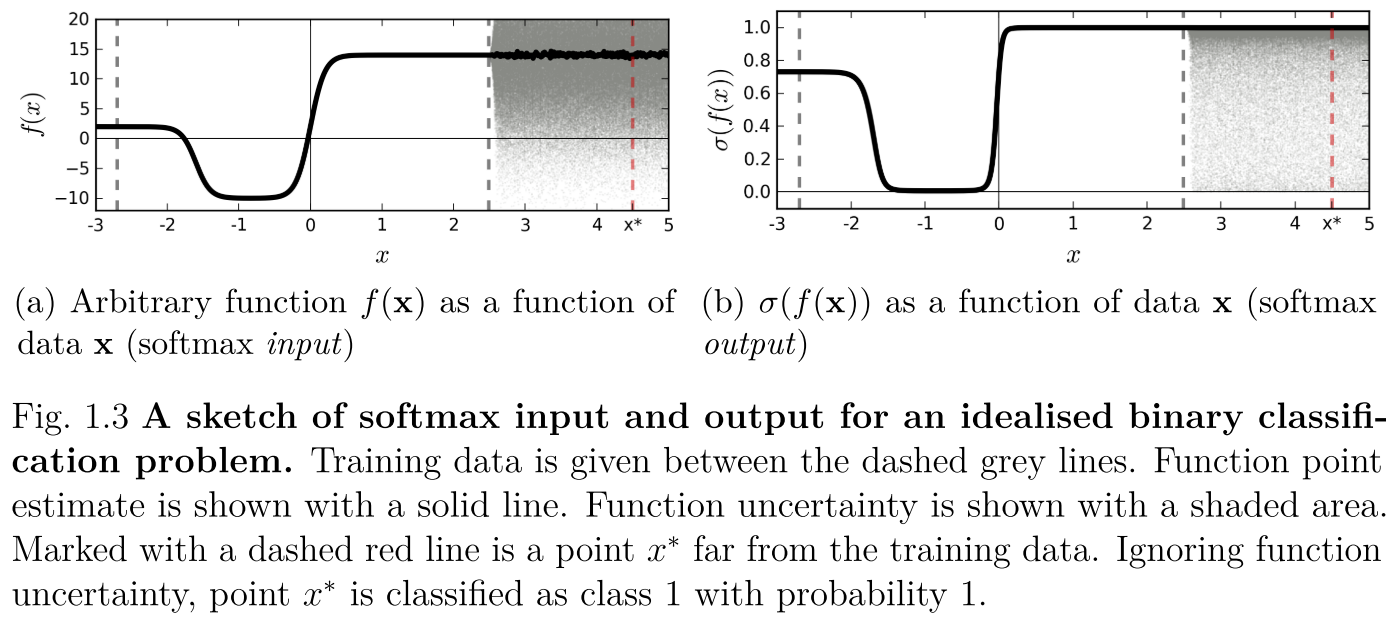
\includegraphics[height=4.5cm]{presentaciones/img/softmax.png}
        \end{center}
    } 

    \uncover<2->{
        \begin{alertblock}{Concepto erróneo}
            El output del modelo \textbf{no equivale} a la incerteza del modelo.
        \end{alertblock}
    } 

   
\end{frame}

\begin{frame}{Objetivo}
    Obtener la \textbf{incerteza} de una red neuronal, mediante un modelo que:
    \begin{itemize}
        \item sea escalable para datasets grandes,
        \item sea escalable para modelos complejos (CNN, RNN, etc.),
        \item use modelos ya existentes y
        \item sea fácil de entender y usar para personas no expertas.
    \end{itemize}
\end{frame}


%%%%%%%%%%%%%%%%%%%%%%%%%%%%%%%%%%%%%%%%%%%%%%%%%%%%%%%%%%%%%%%%%%%%%%
%%%%%%%%%%%%%%%%%%%%%%%%%%%%%%%%%%%%%%%%%%%%%%%%%%%%%%%%%%%%%%%%%%%%%%

\section{Modelamiento bayesiano}

\begin{frame}{Modelamiento bayesiano}
    Dadas las observaciones $\bX, \bY$ se desea encontrar los parámetros $\bomega$ tal que $\by \approx \fb^{\bomega}(\bx)$. Para esto se intenta \textbf{maximizar} la posterior:
    \begin{equation}
        p(\bomega|\bX,\bY) = \dfrac{p(\bY|\bX,\bomega)p(\bomega)}{p(\bY|\bX)},
    \end{equation}
    
    Utilizando esto se puede realizar una predicción utilizando un nuevo punto $\bx^*$ integrando
    \begin{equation}
        p(\by^* | \bx^*, \bX, \bY) = \int p(\by^* | \bx^*, \bomega) p(\bomega | \bX, \bY) \dif \bomega
    \end{equation}
    
    Por lo general, la expresión $p(\bomega|\bX,\bY)$ es intratable, con lo que se utilizará inferencia variacional para obtener una aproximación.
    
    % siendo $p(\bY|\bX)$ la \textbf{evidencia}, dada por:
    
    % \begin{equation}
    %     p(\bY|\bX) = \int p(\bY|\bX,\bomega) p(\bomega) d\bomega.
    % \end{equation}
    
    % Sin embargo, en general esta integral no puede ser calculada analíticamente. Por lo tanto, se requiere una \textbf{aproximación}.
\end{frame}

\subsection{Inferencia variacional}

\begin{frame}{Inferencia variacional}


    \uncover<1->{
    Se define una \textbf{distribución variacional aproximada} $q_\theta(\bomega)$ parametrizada por $\theta$, cuya estructura sea fácil de evaluar.
    \begin{equation}
        q^*_\theta(\bomega) = \argmin_\theta \ \KL\{q_\theta(\bomega)||p(\bomega|\bX,\bY)\}
    \end{equation}
   } 

    \uncover<2->{
     Esto es equivalente a maximizar la \textbf{cota inferior de la evidencia (ELBO)}:
    \vspace{-5pt}
    \begin{equation}
        \ELBO(q) = \esp_{q_\theta(\bomega)}\{\ \log p(\bY|\bX,\bomega)\} - \KL\{q_\theta(\bomega)|| p(\bomega)\} := \L_{\VI}(\theta)
    \end{equation}
   } 
    
    \uncover<3->{
      \begin{exampleblock}{Ventajas}
        \begin{itemize}
            \item Balance: complejidad vs. ajuste de los datos.
            \item Captura la incerteza del modelo.
        \end{itemize}
    \end{exampleblock}
   } 
    
    
\end{frame}


%%%%%%%%%%%%%%%%%%%%%%%%%%%%%%%%%%%%%%%%%%%%%%%%%%%%%%%%%%%%%%%%%%%%%%
%%%%%%%%%%%%%%%%%%%%%%%%%%%%%%%%%%%%%%%%%%%%%%%%%%%%%%%%%%%%%%%%%%%%%%

\section{Bayesian Deep Learning}

\begin{frame}{Bayesian Neural Networks (BNN)}
    En una Red Neuronal Bayesiana se modelan los pesos por medio de una distribución. 
    % Es decir, dadas las matrices de pesos $\bW_i$ y vectores de bias $\bb_i$ para la capa $i$, se asume un prior sobre las matrices de pesos, $p(\bW_i) = \N(\bm{0}, \bm{I})$
    \begin{figure}[H]
        \centering
        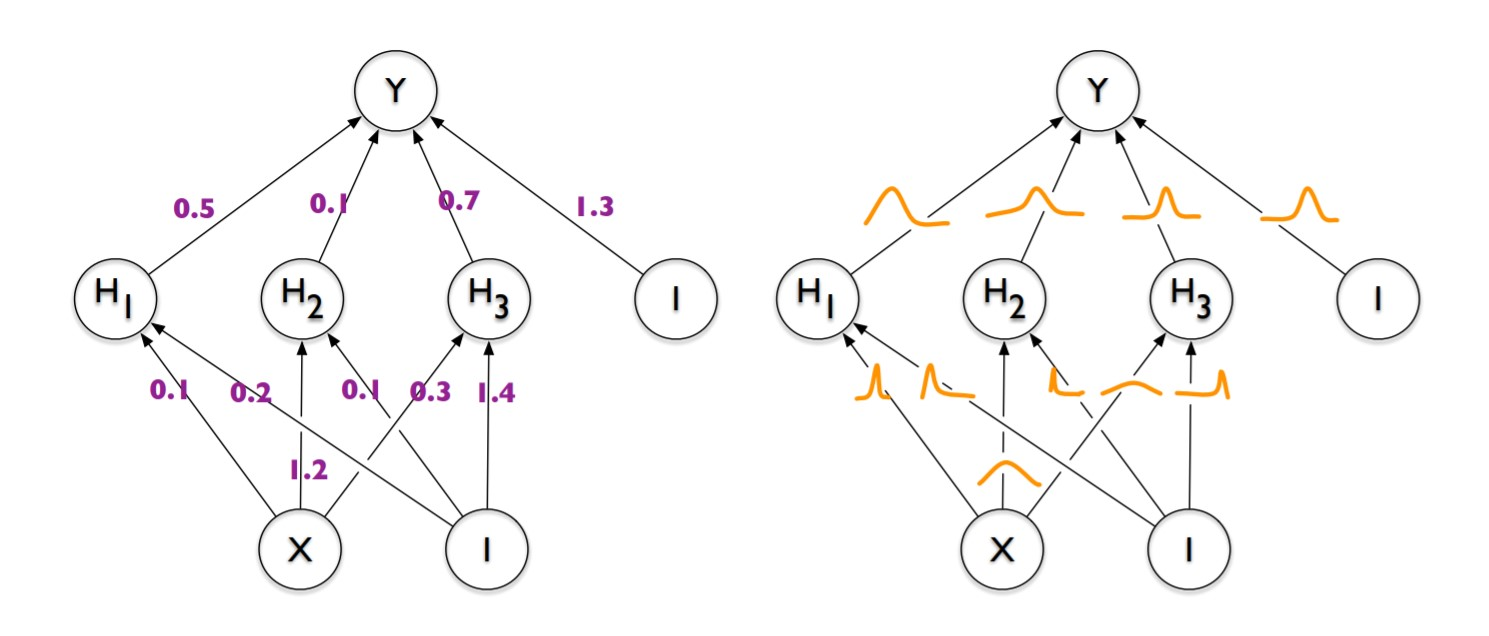
\includegraphics[width=\linewidth]{presentaciones/img/comp_NN_con_BNN.jpg}
        \caption{Comparación de una red neuronal con una red neuronal bayesiana. Obtenido de \cite{blundell2015weight}.}
        \label{fig:comp_NN_con_BNN}
    \end{figure}
\end{frame}

\begin{frame}{Inferencia Variacional en una BNN}
    Recordar que se está buscando la distribución posterior de los pesos dados los datos: $p(\bomega | \bX, \bY)$. Cómo esta expresión es intratable, se aproxima a través de inferencia variacional. Consideramos a la distribución variacional aproximada $q_\theta(\bomega)$ como
    \begin{equation}
        q_\theta(\bomega) = \prod_{i=1}^{L} q_\theta (\bW_i) = \prod_{i, j, k} \N(w_{ijk}; m_{ijk}, \sigma^2_{ijk})
    \end{equation}
    
    Dónde el parámetro $\bomega = \{\bW_i, \bb_i\}_{i=1}^{L}$ corresponde a los pesos y bias de la red
\end{frame}

\begin{frame}{Bayesian Neural Networks (BNN)}
    
    Se considera un prior sobre los pesos de la NN, induciendo una distribución sobre un conjunto paramétrico de funciones.
    \begin{align}
        \begin{split}
            \L_{\VI}(\theta) &= \esp_{q_\theta(\bomega)}\{\log p(\bY|\bX,\bomega)\} - \KL\{q_\theta(\bomega)|| p(\bomega)\} \\
            &= \sum_{i=1}^N \esp_{q_\theta(\bomega)}\{\log p(\by_i|\fb^\bomega(\bx_i))\} - \KL\{q_\theta(\bomega)|| p(\bomega)\},
        \end{split}
    \end{align}

    siendo $\fb^\bomega(\bx_i)$ el output del modelo para $\bx_i$.
    
    
    \begin{exampleblock}{Ventajas}
        \begin{itemize}
            \item Robustos a overfitting.
            \item Estimación de la incerteza.
            \item Puede aprender con datasets pequeños.
        \end{itemize}
    \end{exampleblock}
\end{frame}


\begin{frame}{Bayesian Neural Networks (BNN)}


    \uncover<1->{
        \color{red} \textbf{¡PERO!} \color{black} Esta expresión de $\L_{\VI}(\theta)$:

        \begin{enumerate}
            \item requiere calcular sobre todo el dataset $\Rightarrow$ costoso, e
            \item intratable para modelos complejos (por ej. BNN con más de una capa).
        \end{enumerate}    
    } 
   
    \vspace{10pt}
    \uncover<2->{
        \color{green}
        \textbf{Solución:}
        \color{black}
        
        \begin{enumerate}[<+->]
            \item Usar minibatches.
            \begin{equation}
                \hat{\L}_{\VI}(\theta) = \dfrac{N}{M}\sum_{i\in \mathcal{S}} \esp_{q_\theta(\bomega)}\{\log p(\by_i|\fb^\bomega(\bx_i))\} - \KL\{q_\theta(\bomega)|| p(\bomega)\}
            \end{equation}
            
            \item Usar estimadores Monte Carlo.
    \end{enumerate}    
    } 
   
\end{frame}


\subsection{Monte Carlo}

\begin{frame}{Estimadores de Monte Carlo}

    \uncover<1->{
    \textbf{Objetivo:}
    \begin{itemize}
        \item Estimar la esperanza de la log-likelihood.
        \item Estimar la derivada de la esperanza de la log-likelihood (c/r a $\theta$).
    \end{itemize}
   } 
    
    \vspace{10pt}
    \uncover<2->{
    Existen estimadores para calcular:
    \begin{equation}\label{eq:est}
        I(\theta) = \pd{}{\theta} \esp_{p_\theta(x)} [f(x)]
    \end{equation}
    
    Algunos de estos son:
    \begin{enumerate}
        \item Score function estimator
        \item Pathwise derivative estimator
        \item Characteristic function estimator 
    \end{enumerate}
    }
    
    
\end{frame}

\begin{frame}{Pathwise derivative estimator}
    Entre todos los estimadores, uno de los más útiles es el \textit{Pathwise derivative estimator}. Éste consiste en reparametrizar $p_\theta(x)$ por $p(\epsilon)$ tal que $x = g(\theta, \epsilon)$. De esta forma, se estima \eqref{eq:est} por medio de
    \begin{equation}
        \hat{I}(\theta) = f'(g(\theta, \epsilon)) \pd{}{\theta} g(\theta, )
    \end{equation}
\end{frame}

\begin{frame}{Inferencia práctica en una BNN}
    Se reparametriza cada $q_{\theta_{l, i}}(\bw_{l, i})$ como $\bw_{l, i} = g(\theta_{l, i}, \epsilon_{l, i})$ especificando algún $p(\epsilon_{l, i})$. Con esto, se reparametriza $\hat{\L}_{\VI}$ con respecto a $p(\bepsilon)$
    \begin{align*}
        \hat{\L}_{\VI}(\theta) &= -\frac{N}{M} \sum_{i \in S} \esp_{q_\theta(\bomega)} [\log p(\by_i | \fb^\bomega(\bw_i))] + \KL(q_\theta(\bomega) \| p(\bomega))\\
        &= -\frac{N}{M} \sum_{i \in S} \esp_{p(\bepsilon)} [\log p(\by_i | \fb^{g(\theta, \bepsilon)}(\bw_i))] + \KL(q_\theta(\bomega) \| p(\bomega))
    \end{align*}
    
    Y aplicando la estimación anterior obtenemos que
    \begin{equation}\label{Lmc}
        \hat{\L}_{\MC}(\theta) = -\frac{N}{M} \sum_{i \in S} \log(\by_i | \fb^{g(\theta, \bepsilon)}(\bx_i)) + \KL(q_\theta(\bomega) \| p(\bomega))
    \end{equation}
\end{frame}

\begin{frame}{Algoritmo}
    Aquí quizás ponemos el algoritmo (?) y explicar lo de la Eq. (3.8)
\end{frame}

\subsection{Stochastic Regularization Techniques}

\begin{frame}{Técnicas de regularización Estocástica (SRT)}

¿Qué es una Técnica de Regularización Estocástica?:

\begin{itemize}
    \item Son técnicas de regularización usadas, principalmente, en modelos de DL.
    \item Hacen uso de ruido estocástico para la inyección de este en el modelo a regularizar.
    \item Dos de las técnicas más conocidas son: \textbf {Dropout} y \textbf{Multiplicative Gaussian Noise}
\end{itemize}

\end{frame}

\begin{frame}{SRT como inferencia aproximada}

A diferencia de las SRT, las estocasticidad de las BNN's provienen de los parámetros del modelo. Luego, una forma de transformar el ruido de dropout desde el espacio de características al espacio de parámetros es:
\begin{align*}
    \hat{y} &= \hat{h}\mathbf{M_2} \\
            &= (h \odot \hat{\epsilon_2})M_2\\
            &= (h \cdot diag(\hat{\epsilon_2}))M_2\\
            &= \sigma(\hat{x}M_1 + b)(diag(\hat{\epsilon_2})M_2)\\
            &= \sigma(x(diag(\hat{\epsilon}_1)M_1 + b))(diag(\hat{\epsilon_2})M_2)\\
            &= \sigma(x\hat{W}_1 + b)\hat{W}_2 \eqqcolon f^{\hat{W}_1, \hat{W}_2, b}(x)
\end{align*}

Donde $ {\scriptstyle \hat{W}_1 \coloneqq diag(\hat{\epsilon}_1)M_1}$ y ${\scriptstyle \hat{W}_2 \coloneqq diag(\hat{\epsilon_2})M_2}$
\end{frame}

\begin{frame}{SRT como inferencia aproximada}

Junto a lo anterior y teniendo en cuenta la función objetivo de optimización de una red neuronal, se tiene una función de optimización para una red neuronal con dropout de la siguiente forma:
\begin{multline}\label{Ldrop}
    \hat{\mathcal{L}_{d}}(M_1, M_2, b) \\
    \coloneqq \frac{1}{M}\sum_{i \in S} E^{\hat{W}_1^i, \hat{W}_2^i, b}(x_i, y_i) + \lambda_1 ||M_1||^2 + \lambda_2 ||M_2||^2 + \lambda_3 ||b||^2 
\end{multline}

Donde ${\scriptstyle E^{\hat{W}_1^i, \hat{W}_2^i, b} = \frac{1}{2}||y - f^{\hat{W}_1, \hat{W}_2, b}(x)||^2} = \underbrace{{\scriptstyle-\frac{1}{\tau}\log{p(y|f^{\hat{W}_1, \hat{W}_2, b}(x))} + const}}_{\textcolor{red}{regresión}}$
\end{frame}

\begin{frame}{SRT como inferencia aproximada}

Reemplazando la última expresión en \ref{Ldrop} y agrupando los parámetros en ${\scriptstyle \hat{w_i}
= \{ \hat{W}_1^i, \hat{W}_2^i, b\} = \{ diag(\hat{\epsilon}_1^i)M_1, diag(\hat{\epsilon}_2^i)M_2, b\} \eqqcolon g(\theta, \hat{\epsilon}_i)}$ se reescribe la ecuación \ref{Ldrop} como:
\begin{multline}\label{Ldrop2}
    % {\scriptstyle \hat{\mathcal{L}}_{d}(M_1, M_2, b) = \frac{1}{M\tau}\sum_{i \in S}\log{p(y_i|f^{g(\theta, \hat{\epsilon}_1)}(x))} + \lambda_1||M_1||^2 + \lambda_2||M_2||^2 + \lambda_3||b||^2}  
    {\hat{\mathcal{L}}_{d}(M_1, M_2, b) = \\
    \frac{1}{M\tau}\sum_{i \in S}\log{p(y_i|f^{g(\theta, \hat{\epsilon}_1)}(x))} + \lambda_1||M_1||^2 + \lambda_2||M_2||^2 + \lambda_3||b||^2}  
\end{multline}

Esta última ecuación y la ecuación de perdida \ref{Lmc} son similares, salvo las siguientes diferencias:

\begin{itemize}
    \item Los términos derivativos de regularización ${\scriptstyle KL(q_{\theta}(\bomega)||p(\bomega))}$ en \ref{Lmc} y ${\scriptstyle \lambda_1||M_1||^2 + \lambda_2||M_2||^2 + \lambda_3||b||^2}$ en \ref{Ldrop2} 
    \item Términos de escala.
\end{itemize}
\end{frame}

\begin{frame}{MC vs Dropout}

Finalmente, si se define el prior $p(\omega)$ sujeto a la condición \ref{kl_cond}:
\begin{equation}\label{kl_cond}
    \scalebox{0.9}{$\frac{\partial}{\partial \theta} KL(q_{\theta}(\omega) || p(\omega)) = \frac{\partial}{\partial \theta} N\tau (\lambda_1||M_1||^2 + \lambda_2||M_2||^2 + \lambda_2||b||^2)$}
\end{equation}

Se llega a la siguiente relación:
\begin{equation}\label{mc-drop}
\frac{\partial}{\partial \theta}\hat{\mathcal{L}}_{d}(\theta) = \frac{1}{N\tau}\frac{\partial}{\partial \theta} \hat{\mathcal{L}}_{MC}(\theta)
\end{equation}
\textbf{\textcolor{black}{Poseen el mismo procedimiento de optimización!}}
\end{frame}
\begin{frame}{SRTs}
     \begin{block}{Interpretación}
        Optimizar \textbf{cualquier} NN con dropout es \textbf{equivalente} a una forma de inferencia aproximada: los pesos óptimos de un dropout NN son los mismos que los parámetros variacionales óptimos de una BNN con la misma estructura.
    \end{block}
    
    \begin{alertblock}{¿Qué significa?}
    Que las NN entrenadas con dropout poseen todas las \textbf{propiedades} que posee una BNN.
    \end{alertblock}
\end{frame}

\subsection{Model Uncertainty in BNN}

\begin{frame}{Model Uncertainty in BNN}

\begin{block}{Proposición 2}

Dado $p(y^*| f^{w}(x^*)) = \mathcal{N}(y^*; f^{w}(x^*), \tau^{-1}I)$, se puede estimar $\mathbb{E}_{q_{\theta}^* (y^*|x^*)}[y^*]$ con el siguiente estimador:

$$\tilde{\mathbb{E}}[y^*] \coloneqq \frac{1}{T}\sum_{t=1}^{T} f^{\hat{w}_t}(x^*) \xrightarrow[T \to \infty]{} \mathbb{E}_{q_{\theta}^* (y^*|x^*)}[y^*]$$
   
\end{block}

\end{frame}

\subsection{Análisis}

\begin{frame}{Análisis}
    un analisis
\end{frame}



%%%%%%%%%%%%%%%%%%%%%%%%%%%%%%%%%%%%%%%%%%%%%%%%%%%%%%%%%%%%%%%%%%%%%%
%%%%%%%%%%%%%%%%%%%%%%%%%%%%%%%%%%%%%%%%%%%%%%%%%%%%%%%%%%%%%%%%%%%%%%

\section{Demo}

\begin{frame}{Demo}
    \begin{figure}[H]
        \centering
        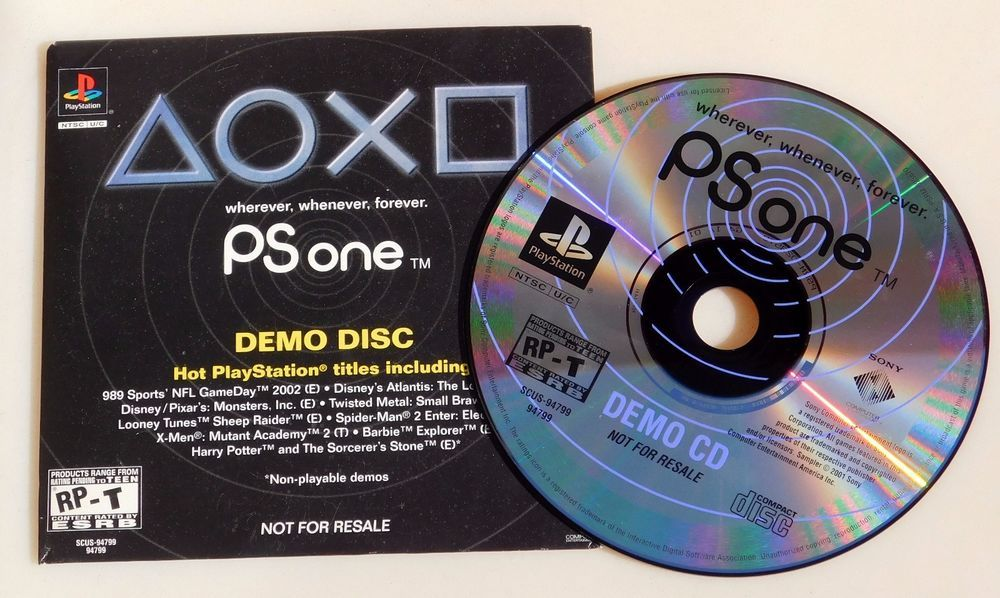
\includegraphics[scale=0.2]{presentaciones/img/demopsx.jpg}
        \caption{Psx Demo}
        \label{psx}
    \end{figure}
\end{frame}

\section{Conclusión}

\begin{frame}{Conclusión}
    conclusiones
\end{frame}


\begin{frame}{Conclusión}
    \centering
    \Huge ¡Gracias!
\end{frame}

% \begin{frame}{Referencias}
%     \printbibliography
% \end{frame}

\begin{frame}{Tercera diapo}
    AQUÍ HAY MÁS INFO
     \begin{block}{Primer bloque}
        Aquí está el primer bloque
    \end{block}
    \begin{exampleblock}{Bloque de ejemplo}
        Aquí hay un bloque de ejemplo
    \end{exampleblock}
    \begin{alertblock}{Bloque de alerta}
        Aquí hay un bloque de alerta
    \end{alertblock}
\end{frame}
